\documentclass[t]{beamer}

\mode<presentation>
{
  \usetheme{default}
  \setbeamertemplate{navigation symbols}{}
  \setbeamertemplate{footline}[frame number]
  \setbeamertemplate{items}[circle]
  \usecolortheme{seahorse}
}

\usepackage[english]{babel}
\usepackage[utf8]{inputenc}
\usepackage{times}
\usepackage[T1]{fontenc}
\usepackage{url}
\usepackage{amsmath}

\parskip=8 pt

\newcommand\topstrut{\rule{0pt}{2.6ex}}
\newcommand\bottomstrut{\rule[-1.2ex]{0pt}{0pt}}
\newcommand\doublestrut{\rule[-1.2ex]{0pt}{3.6ex}}

\newcommand\blue[1]{\textcolor{blue}{#1}}
\newcommand\gray[1]{\textcolor{gray}{#1}}
\newcommand\smallgray[1]{\textcolor{gray}{\small\it #1}}
\newcommand\prevwork[1]{\smallgray{#1}}

\title[WTF?] % (optional, only for long titles)
{WTF is Deep Learning}
\subtitle{A brief history}

\author[Abrahamson] {Jeff Abrahamson} \institute[Google]{Google,
  Inc.\\{\tiny\it The views expressed in these slides are the author's
    and do not necessarily reflect those of Google.}}

\date[Deep Learning Meetup]
{London Deep Learning Meetup, 9 July 2014}

% Delete this, if you do not want the table of contents to pop up at
% the beginning of each subsection:
\AtBeginSubsection[]
{
  \begin{frame}<beamer>{Outline}
    \tableofcontents[currentsection,currentsubsection]
  \end{frame}
}

% If you wish to uncover everything in a step-wise fashion, uncomment
% the following command: 
%\beamerdefaultoverlayspecification{<+->}

\begin{document}

\begin{frame}
  \titlepage
\end{frame}

\begin{frame}
  \frametitle{Outline}
  \tableofcontents
\end{frame}

\section{Overview}
%\subsection{Subsection}

\begin{frame}
  \frametitle{Roughly, wtf is Deep Learning?}
  \begin{itemize}
  \item<1-> Machine learning
  \item<1-> Model high-level abstraction by using multiple non-linear
    transformations.
  \item<2-> Example: \blue{Image:}
  \end{itemize}
  \only<2>{\centerline{\blue{pixels $\Rightarrow$ edges $\Rightarrow$ shapes
    $\Rightarrow$ faces.}}}
\end{frame}

\begin{frame}
  \frametitle{Review}
  Broadly, ML comes in three flavors:
  \begin{itemize}
  \item \blue{Supervised learning:} Predict output given input
  \item \blue{Reinforcement learning:} Select action to maximize payoff
  \item \blue{Unsupervised learning:} Discover a good internal
    representation of input
  \end{itemize}
\end{frame}

\begin{frame}
  \frametitle{Review}
  Supervised learning comes in two flavors:
  \begin{itemize}
  \item \blue{Regression:} real-valued output
  \item \blue{Classification:} labeled output
  \end{itemize}
\end{frame}

\begin{frame}
  \frametitle{Review}
  The idea behind supervised learning is often written thus:
  \begin{displaymath}
    y = f(x,W)
  \end{displaymath}
  \only<2>{
    where
    \begin{align*}
      y &= \text{predicted output} \\[2mm]
      x &= \text{input} \\[2mm]
      W &= \text{parameters}
    \end{align*}
    \blue{and our goal is to adjust parameters to minimize loss (error)}
  }
\end{frame}

\begin{frame}
  \frametitle{Review}
  Unsupervised learning
  \begin{itemize}
  \item<1-> Historically, it's clustering
  \item<1-> Now we can do more
  \item<2-> \blue{Create an internal representation of the input that
      is useful for later supervised or reinforcement learning}
  \item<2->\blue{Find a compact, low-dimensional representation of the input}
  \end{itemize}
\end{frame}

\begin{frame}
  \frametitle{Some architectures}
  \begin{itemize}
  \item Deep neural networks
  \item Convolutional deep neural networks
  \item Deep belief networks
  \end{itemize}
\end{frame}

\begin{frame}
  \frametitle{Some successful applications}
  \begin{itemize}
  \item Computer vision (CV)
  \item Speech recognition (ASR)
  \item Natural language processing (NLP)
  \item Music and audio recognition
  \end{itemize}
\end{frame}

\begin{frame}
  \frametitle{Some famous data sets}
  \begin{itemize}
  \item TIMIT (ASR)
  \item MNIST (image classification)
  \item ImageNet
  \end{itemize}
  \note{ImageNet is 1.3 million high-resolution training images}
\end{frame}

\begin{frame}
  \frametitle{Some successful hardware}
  \begin{itemize}
  \item GPU's
  \item Data centers
  \end{itemize}
  
  \prevwork{Luiz André Barroso and Urs Hölzle, The Datacenter as a
    Computer: An Introduction to the Design of Warehouse-Scale
    Machines, 2009.}
\end{frame}

\begin{frame}
  \frametitle{GPU's}
  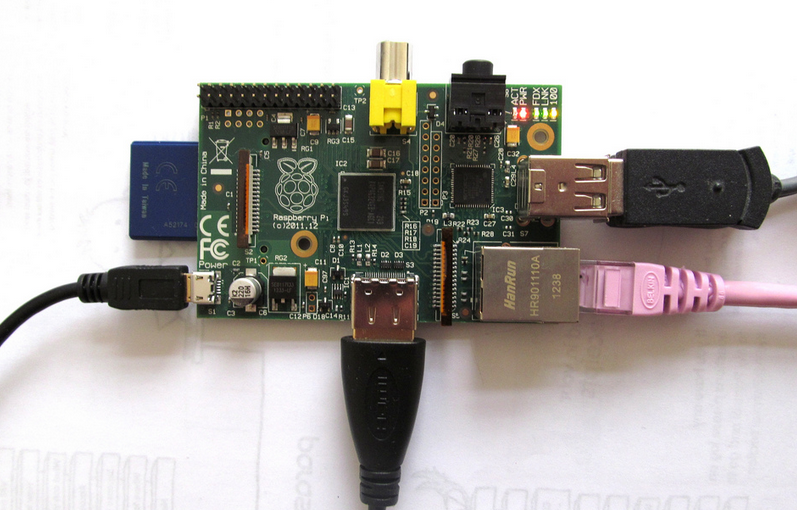
\includegraphics[width=.9\textwidth]{raspberry-pi.png}

  \prevwork{\url{http://petewarden.com/2014/06/09/deep-learning-on-the-raspberry-pi/}}
  \note{Ported Deep Belief image recognition SDK to the raspberry pi}
\end{frame}

\begin{frame}
  \frametitle{What is Hello World for GPU's?}
  Some things to look at.  \gray{(Disclaimer: I haven't.)}
  \begin{itemize}
  \item CUDA (but only nvidia) \hspace{3mm}\gray{\url{www.nvidia.com/object/cuda_home_new.html}}
  \item OpenCL (originally Apple) \hspace{3mm}\gray{\url{https://en.wikipedia.org/wiki/OpenCL}}
  \item GPU++ / GPGPU \hspace{3mm}\gray{\url{http://gpgpu.org/}}
  \item libSh \hspace{3mm}\gray{\url{http://libsh.org/}}
  \item OpenACC \hspace{3mm}\gray{\url{http://www.openacc-standard.org/}}
  \end{itemize}
\end{frame}

\begin{frame}
  \frametitle{Data Centers}
  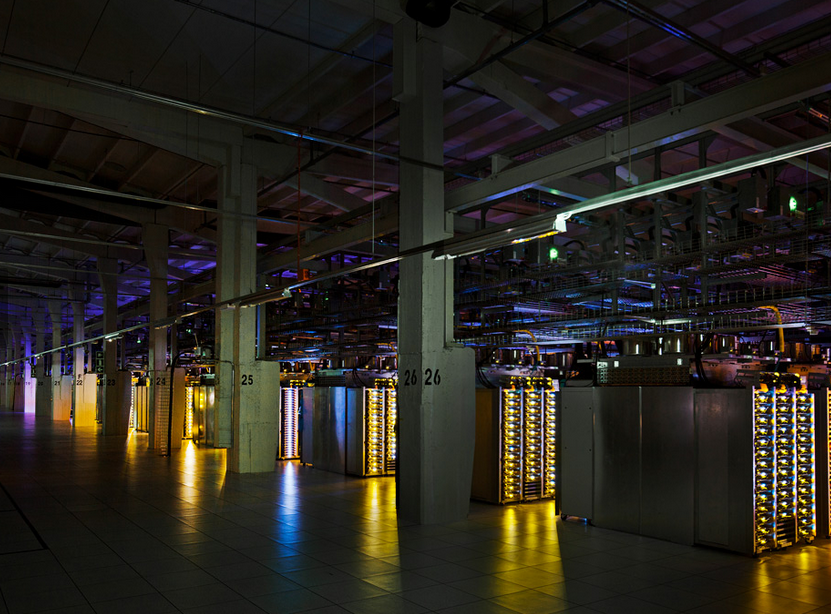
\includegraphics[width=.9\textwidth]{google-dc.png}

  \prevwork{\url{https://www.google.com/about/datacenters/}}
\end{frame}

\section{WTF is a neural Network?}

\begin{frame}
  \frametitle{Why ML at all?}
  \begin{itemize}
  \item We don't know how \textit{we} do it
  \item Write programs to write programs
  \end{itemize}
\end{frame}

\begin{frame}
  \frametitle{Brains (yum!)}
  \begin{itemize}
  \item Neurons, synapses, chemistry
  \item Special kind of parallelism
  \item Power (but we're not there yet)
  \end{itemize}
\end{frame}

\begin{frame}
  \frametitle{Neurons}
  \vspace{2cm}
  \centerline{\huge A brief tour of some neurons}
\end{frame}

\begin{frame}
  \frametitle{Linear neuron}
  \begin{displaymath}
    y = b + \sum_i x_i w_i
  \end{displaymath}
  \only<2>{where
    \begin{align*}
      y & = \text{output} \\
      b & = \text{bias} \\
      x_i & = \text{$i^\mathrm{\,th}$ input} \\
      w_i & = \text{weight on $i^\mathrm{\,th}$ input}
    \end{align*}
  }
  \includegraphics<3>[width=.7\textwidth]{linear-neuron.pdf}
\end{frame}

\begin{frame}
  \frametitle{Binary threshold neuron}
  \begin{align*}
    z & = \sum_i x_i w_i \\[2mm]
    y & = \left\{
      \begin{array}{l}
        1  \text{ if } z \ge 0 \\
        0  \text{ otherwise}        
      \end{array}
    \right.
  \end{align*}
  \only<2>{
    where
    \begin{align*}
      z & = \text{total input} \\
      y & = \text{output} \\
      x_i & = \text{$i^\mathrm{\,th}$ input} \\
      w_i & = \text{weight on $i^\mathrm{\,th}$ input}
    \end{align*}
    \prevwork{W. McCulloch and W. Pitts, A logical calculus
      of the ideas immanent in nervous activity. Bulletin of
      Mathematical Biophysics, 7:115--133, 1943.}
  }
  \includegraphics<3>[width=.7\textwidth]{binary-threshold-neuron.pdf}
\end{frame}

\begin{frame}
  \frametitle{Rectified linear neuron}
  \begin{align*}
    z & = b + \sum_i x_i w_i \\[2mm]
    y & = \left\{
      \begin{array}{l}
        z  \text{ if } z \ge 0 \\
        0  \text{ otherwise}        
      \end{array}
    \right.
  \end{align*}
  \only<2>{
    where
    \begin{align*}
      z & = \text{total input} \\
      y & = \text{output} \\
      b & = \text{bias} \\
      x_i & = \text{$i^\mathrm{\,th}$ input} \\
      w_i & = \text{weight on $i^\mathrm{\,th}$ input}
    \end{align*}
  }
  \includegraphics<3>[width=.7\textwidth]{rectified-linear-neuron.pdf}
\end{frame}

\begin{frame}
  \frametitle{Sigmoid neuron}
  \begin{align*}
    z & = b + \sum_i x_i w_i \\[2mm]
    y & = \frac{1}{1+e^{-z}}
  \end{align*}
  \only<2>{
    \blue{(It's differentiable!)}
  }
  \includegraphics<3>[width=.7\textwidth]{sigmoid-neuron.pdf}
\end{frame}

\begin{frame}
  \frametitle{Stochastic binary neuron}
  \begin{align*}
    z & = b + \sum_i x_i w_i \\[2mm]
    p &= \frac{1}{1+e^{-z}} \\[3mm]
    y & = \left\{
      \begin{array}{l}
        1  \text{ with probability } p \\[2mm]
        0  \text{ with probability } 1 - p
      \end{array}
    \right.
  \end{align*}
  \only<2>{\blue{(a probability distribution)}}

  \only<3>{\blue{Can also do something similar with rectified linear
      neurons, produce spikes with probability $p$ with a Poisson
      distribution.}}
\end{frame}

\begin{frame}
  \frametitle{Example: handwriting recognition of digits}
  \vspace{2cm}
  \centerline{\huge A (too) quick example}
\end{frame}

\begin{frame}
  \frametitle{Example: handwriting recognition of digits}
  \begin{itemize}
  \item<1-> Input neurons: pixels
  \item<1-> Output neurons: classes (digits)
  \item<1-> Connect them all! \textit{(bipartite)}
  \item<2-> Initialize input weights to random
  \end{itemize}
  \includegraphics<3>[width=.4\textwidth]{input-weights.jpg}
\end{frame}

\begin{frame}
  \frametitle{Example: handwriting recognition of digits}
  To train this ANN:
  \begin{itemize}
  \item<1-> Increment weights from active pixels going to correct class
  \item<1-> Decrement weights from active pixels going to predicted class
  \end{itemize}
  \only<2->{When it's right, nothing happens.  This is good.}
\end{frame}

\section{History}

\begin{frame}
  \frametitle{Some inspirations}
  \begin{itemize}
  \item Biology: David H. Hubel and Torsten Wiesel (1959) found two
    types of cells in the visual primary cortex: simple and complex.
  \item Cascading models
  \end{itemize}

  \prevwork{M Riesenhuber, T Poggio. Hierarchical models of object
    recognition in cortex. Nature neuroscience, 1999(11) 1019–1025.}
\end{frame}

\begin{frame}
  \frametitle{History}
  \begin{itemize}
  \item<1-> ANN's exist pre-1980.  Backpropagation since 1974.
  \item<2-> Neocognitron (Kunihiko Fukushima, 1980), partially unsupervised
    % https://en.wikipedia.org/wiki/Neocognitron
  \item<3-> Yann LeCun et al. recognize handwritten postal codes (backpropagation)
  \end{itemize}
  \note{LeCun: But it took 3 days to train, so was not practical for
    general use.}
  
  \only<1>{\prevwork{P. Werbos., ``Beyond Regression: New Tools for
      Prediction and Analysis in the Behavioral Sciences,'' PhD thesis,
      Harvard University, 1974.}}
  
  \only<2>{\prevwork{K. Fukushima., ``Neocognitron: A self-organizing
      neural network model for a mechanism of pattern recognition
      unaffected by shift in position,'' Biol. Cybern., 36, 193–202,
      1980.}}
  
  \only<3>{\prevwork{LeCun et al., ``Backpropagation Applied to
      Handwritten Zip Code Recognition,'' Neural Computation, 1,
      pp. 541–551, 1989.}}
\end{frame}

\begin{frame}
  \frametitle{Paradise glimpsed, paradise lost}
  \begin{itemize}
  \item ANN's were slow.
  \item Vanishing gradient problem (Sepp Hochreiter)
  \item Support vector machines (SVN) were faster
  \end{itemize}
  \note{For two decades from 1990 or so, the world preferred SVN's.}

\prevwork{S. Hochreiter., ``Untersuchungen zu dynamischen neuronalen
  Netzen,'' Diploma thesis. Institut f. Informatik, Technische
  Univ. Munich. Advisor: J. Schmidhuber, 1991.}

\prevwork{S. Hochreiter et al., ``Gradient flow in recurrent nets: the
  difficulty of learning long-term dependencies,'' In S. C. Kremer and
  J. F. Kolen, editors, A Field Guide to Dynamical Recurrent Neural
  Networks. IEEE Press, 2001.}
\end{frame}

\begin{frame}
  \frametitle{Some progress} 

  Multi-level hierarchy of networks (pre-train by level, unsupervised,
  backpropagation) (1992)

  \prevwork{J. Schmidhuber., ``Learning complex, extended sequences
    using the principle of history compression,'' Neural Computation,
    4, pp. 234–242, 1992.}
\end{frame}

\begin{frame}
  \frametitle{Some progress}
    
  Long short term memory network (LSTM) (1997)

  \prevwork{Hochreiter, Sepp; and Schmidhuber, Jürgen; Long
    Short-Term Memory, Neural Computation, 9(8):1735–1780, 1997.}
\end{frame}

\begin{frame}
  \frametitle{Some progress} 

  Deep multidimensional LSTM networks win three ICDAR competitions in
  handwriting recognition without prior language knowledge (2009)

  \prevwork{Graves, Alex; and Schmidhuber, Jürgen; Offline Handwriting
    Recognition with Multidimensional Recurrent Neural Networks, in
    Bengio, Yoshua; Schuurmans, Dale; Lafferty, John; Williams, Chris
    K. I.; and Culotta, Aron (eds.), Advances in Neural Information
    Processing Systems 22 (NIPS'22), December 7th–10th, 2009,
    Vancouver, BC, Neural Information Processing Systems (NIPS)
    Foundation, 2009, pp. 545–552.}

  \prevwork{A. Graves, M. Liwicki, S. Fernandez, R. Bertolami,
    H. Bunke, J. Schmidhuber. A Novel Connectionist System for
    Improved Unconstrained Handwriting Recognition. IEEE Transactions
    on Pattern Analysis and Machine Intelligence, vol. 31, no. 5,
    2009.}
\end{frame}

\begin{frame}
  \frametitle{Some progress}

  Use sign of gradient (Rprop) for image reconstruction and face
  localization (2003)

  \prevwork{Sven Behnke (2003). Hierarchical Neural Networks for Image
    Interpretation.. Lecture Notes in Computer Science
    2766. Springer.}
\end{frame}

\begin{frame}
  \frametitle{And then there was Hinton}
  \begin{itemize}
  \item Geoffrey Hinton and Ruslan Salakhutdinov
  \item Train many-layered feedforward NN's one layer at a time
  \item Treat layers as unsupervised restricted Boltzmann machines
    (Smolensky, 1986)
  \item Use supervised backprogagation for label classification
  \item \gray{Also: Schmidhuber and recurrent NN's}
  \end{itemize}
\end{frame}

\begin{frame}
  \frametitle{And then there was Hinton (bibliography)}

\prevwork{G. E. Hinton., ``Learning multiple layers of
  representation,'' Trends in Cognitive Sciences, 11, pp. 428–434,
  2007.}

\prevwork{J. Schmidhuber., ``Learning complex, extended sequences using
  the principle of history compression,'' Neural Computation, 4,
  pp. 234–242, 1992.}

\prevwork{J. Schmidhuber., ``My First Deep Learning System of 1991 +
  Deep Learning Timeline 1962–2013.''}

\prevwork{Smolensky, P. (1986). ``Information processing in dynamical
  systems: Foundations of harmony theory.''. In D. E. Rumelhart,
  J. L. McClelland, and the PDP Research Group, Parallel Distributed
  Processing: Explorations in the Microstructure of
  Cognition. 1. pp. 194–281.}
\end{frame}

\begin{frame}
  \frametitle{And then there was Hinton (bibliography)}

\prevwork{Hinton, G. E.; Osindero, S.; Teh, Y. (2006). ``A fast
  learning algorithm for deep belief nets''. Neural Computation 18 (7):
  1527–1554. doi:10.1162/neco.2006.18.7.1527. PMID 16764513.}

\prevwork{Hinton, G. (2009). ``Deep belief networks''. Scholarpedia 4
  (5): 5947. doi:10.4249/scholarpedia.5947. edit}
\end{frame}

\begin{frame}
  \frametitle{Yet more progress}

  Google Brain project (Andrew Ng, Jeff Dean) recognized cats in
  youtube videos.

  \prevwork{Ng, Andrew; Dean, Jeff (2012). ``Building High-level
    Features Using Large Scale Unsupervised Learning''.}

  \prevwork{John Markoff (25 June 2012). ``How Many Computers to
    Identify a Cat? 16,000.'', New York Times.}

\end{frame}

\begin{frame}
  \frametitle{More progress}
  Brute force!

  Dan Ciresan et al. (IDSIA, 2010) use lots of GPU's to
  bulldoze the vanishing gradient problem and outperform LeCun (and
  everyone else) on MNIST.

  \prevwork{D. C. Ciresan et al., ``Deep Big Simple Neural Nets for
    Handwritten Digit Recognition,'' Neural Computation, 22,
    pp. 3207–3220, 2010.}
\end{frame}

\begin{frame}
  \frametitle{State of the art, 2011}

  Deep learning feedforward networks
  \begin{itemize}
  \item Convolutional layers
  \item Max-pooling layers
  \item Plus pure classification layers
  \end{itemize}

  \prevwork{D. C. Ciresan, U. Meier, J. Masci, L. M. Gambardella,
    J. Schmidhuber. Flexible, High Performance Convolutional Neural
    Networks for Image Classification. International Joint Conference
    on Artificial Intelligence (IJCAI-2011, Barcelona), 2011.}

  \prevwork{Martines, H., Bengio, Y., and Yannakakis,
    G. N. (2013). Learning Deep Physiological Models of Affect. I EEE
    Computational Intelligence, 8(2), 20.}
\end{frame}

\begin{frame}
  \frametitle{State of the art, post-2011}
  
  Lots of GPU's.  Sometimes human-competitive performance!
  \begin{itemize}
  \item IJCNN 2011 Traffic Sign Recognition Competition
  \item ISBI 2012 Segmentation of neuronal structiosn in EM stacks challenge
  \item and more
  \end{itemize}

\end{frame}

\begin{frame}
  \frametitle{State of the art, post-2011}
  
  \prevwork{D. C. Ciresan, U. Meier, J. Masci, L. M. Gambardella,
    J. Schmidhuber. Flexible, High Performance Convolutional Neural
    Networks for Image Classification. International Joint Conference
    on Artificial Intelligence (IJCAI-2011, Barcelona), 2011}

  \prevwork{D. C. Ciresan, U. Meier, J. Masci,
    J. Schmidhuber. Multi-Column Deep Neural Network for Traffic Sign
    Classification. Neural Networks, 2012.}

  \prevwork{D. Ciresan, A. Giusti, L. Gambardella,
    J. Schmidhuber. Deep Neural Networks Segment Neuronal Membranes in
    Electron Microscopy Images. In Advances in Neural Information
    Processing Systems (NIPS 2012), Lake Tahoe, 2012.}

  \prevwork{D. C. Ciresan, U. Meier, J. Schmidhuber. Multi-column Deep
    Neural Networks for Image Classification. IEEE Conf. on Computer
    Vision and Pattern Recognition CVPR 2012.}

\end{frame}

\begin{frame}
  \frametitle{Basic ideas}
  \begin{itemize}
  \item Distributed representations: observed data is organized at
    multiple levels of abstraction or composition
  \item Higher level concepts learned from lower level concepts
    (hierarchical explanatory factors)
  \item Often can frame problems as unsupervised.  (Labeling is
    expensive.)
  \end{itemize}
  
  \prevwork{Y. Bengio, A. Courville, and P. Vincent., ``Representation
    Learning: A Review and New Perspectives,'' IEEE Trans. PAMI,
    special issue Learning Deep Architectures, 2013.}
\end{frame}

\begin{frame}
  \frametitle{Basic ideas}
  \begin{itemize}
  \item Unsupervised $\Rightarrow$ unlabeled data is ok
  \item Often greedy between layers
  \end{itemize}
\end{frame}

\begin{frame}
  \frametitle{}
  \begin{itemize}
  \item 
  \end{itemize}
\end{frame}

\begin{frame}
  \frametitle{}
  \begin{itemize}
  \item 
  \end{itemize}
\end{frame}

\begin{frame}
  \frametitle{}
  \begin{itemize}
  \item 
  \end{itemize}
\end{frame}

\begin{frame}
  \frametitle{}
  \begin{itemize}
  \item 
  \end{itemize}
\end{frame}

\begin{frame}
  \frametitle{}
  \begin{itemize}
  \item 
  \end{itemize}
\end{frame}

\begin{frame}
  \frametitle{}
  \begin{itemize}
  \item 
  \end{itemize}
\end{frame}

\begin{frame}
  \frametitle{}
  \begin{itemize}
  \item 
  \end{itemize}
\end{frame}

\begin{frame}
  \frametitle{}
  \begin{itemize}
  \item 
  \end{itemize}
\end{frame}

\begin{frame}
  \frametitle{}
  \begin{itemize}
  \item 
  \end{itemize}
\end{frame}

\begin{frame}
  \frametitle{}
  \begin{itemize}
  \item 
  \end{itemize}
\end{frame}



\end{document}
